\section{Generalidades de la empresa}
\label{ch:generalidades}

\subsection{Antecedentes históricos}
\label{sec:antecedentes_historicos}

Honne es una empresa especializada en transformación tecnológica, consultoría y gestión de infraestructura de TI que cuenta con más de 8 años de experiencia en el mercado. A lo largo de su trayectoria ha consolidado su operación a nivel internacional, habiendo entregado más de 300 proyectos \cite{honne_oficial_2026}.

Actualmente cuenta con presencia operativa en 6 países: México, Colombia, Chile, Estados Unidos, Francia y España. Su principal Centro de Operación y Excelencia Multicloud (CCoE), donde se operan servicios multicloud, se ubica en Ciudad Victoria, Tamaulipas, sumado a su oficina corporativa en Monterrey y sedes en la Ciudad de México, Bogotá, Santiago, Houston, París y Madrid. Asimismo, ha forjado alianzas de alto nivel como partner de AWS, Google Cloud Platform, Microsoft Azure, Alibaba Cloud, Oracle y NVIDIA \cite{honne_oficial_2026}.

\subsection{Actividad principal, productos o servicios}
\label{sec:giro_actividad}

Según la información institucional de la empresa \cite{honne_oficial_2026}, su actividad principal, así como sus productos y servicios, se describen a continuación.

\textbf{Actividad principal.} Honne es una firma de ingeniería de valor empresarial (\textit{Engineering Enterprise Value}), enfocada en el sector de las Tecnologías de la Información, la consultoría cloud y la gestión de infraestructura. Se dedica a combinar el uso de la nube pública, la Inteligencia Artificial (IA) y las operaciones de TI para alinear la tecnología con los objetivos de negocio de sus clientes, generando un impacto medible y apoyándolos a escalar su infraestructura y operar con estabilidad.

\textbf{Productos o servicios.} Sus soluciones se enmarcan en el modelo \textit{Enterprise Value Framework}, estructurado en las siguientes dimensiones:
\begin{itemize}
    \item \textbf{Stability (Estabilidad):} gestión y monitoreo continuo, mediante plataformas como Google Cloud o AWS, para garantizar una operación estable, segura y controlada que asegure la eficiencia y continuidad del negocio.
    \item \textbf{Modernization (Modernización):} transformación estructural y evolución de la arquitectura tecnológica de los clientes para que puedan crecer con agilidad y sin fricción.
    \item \textbf{Intelligence (Inteligencia):} aplicación de análisis de datos e Inteligencia Artificial para optimizar las operaciones corporativas y fomentar la toma de mejores decisiones.
    \item \textbf{AI Fusion:} práctica dedicada a implementar la IA, llevando modelos desde la fase de piloto hasta su producción real con impacto en el negocio.
\end{itemize}

\subsection{Misión, visión, valores y política de calidad}
\label{sec:mision_vision}

De acuerdo con la información institucional de la empresa \cite{honne_oficial_2026}, la misión de Honne es crear valor para sus clientes mediante la innovación y las Tecnologías de la Información, mientras que su visión es ser líderes mundiales en la gestión de nube pública y en la creación de servicios de próxima generación.

Sus valores fundamentales son:
\begin{itemize}
    \item Confiabilidad
    \item Servicio excepcional
    \item Innovación
    \item Mejora continua
    \item Máxima productividad
\end{itemize}

En cuanto a su política de calidad, Honne opera bajo un ecosistema de estándares y certificaciones internacionales —ISO 9001 (Gestión de la Calidad), ISO 20000 (Gestión de Servicios de TI), ISO 27001 (Seguridad de la Información), ITIL, CMMI (Modelo de Madurez de Capacidades) y TOGAF (Marco de Arquitectura Empresarial)— que garantizan la excelencia operativa en cada entrega. Su compromiso operativo se rige, además, por la filosofía de trabajo \textit{One Team}, que fomenta equipos integrados bajo una sola visión, desde la consultoría inicial hasta el soporte y el monitoreo continuo.

\subsection{Infraestructura general}
\label{sec:infraestructura}

La infraestructura tecnológica de Honne se basa en un modelo multicloud: opera y da soporte a sus clientes sobre las principales plataformas de nube pública (AWS, Microsoft Azure, Google Cloud Platform y Alibaba Cloud), además de soluciones de cómputo empresarial e Inteligencia Artificial con Oracle y NVIDIA \cite{honne_oficial_2026}. Esta operación se centraliza desde el CCoE, que brinda soporte y monitoreo a clientes en México, Estados Unidos, Europa y Latinoamérica \cite{honne_oficial_2026}, apoyándose en las herramientas de monitoreo descritas más adelante en este apartado (correo electrónico, ServiceNow, TIBCO Scribe y Zendesk).

\subsection{Organigrama y ubicación del departamento}
\label{sec:organigrama_ubicacion}

El Centro de Operación y Excelencia Multicloud (CCoE), donde se realizó la Estadía, se ubica en calle 533 Maratines, Ciudad Victoria, Tamaulipas (ver Figura \ref{fig:ubicacion_ccoe}).

\begin{figure}[h]
    \centering
    
\includegraphics[width=0.7\textwidth]{img/figura_ubicacion_ccoe.png}
    \caption{Ubicación del CCoE de Honne en Ciudad Victoria, Tamaulipas.}
    \label{fig:ubicacion_ccoe}
\end{figure}

La Figura \ref{fig:organigrama} muestra la estructura organizacional de Honne. La Estadía se realizó dentro del equipo de Mesa de Servicio, ubicado en la columna de Servicios Administrados 2.0.

\begin{figure}[h]
    \centering
    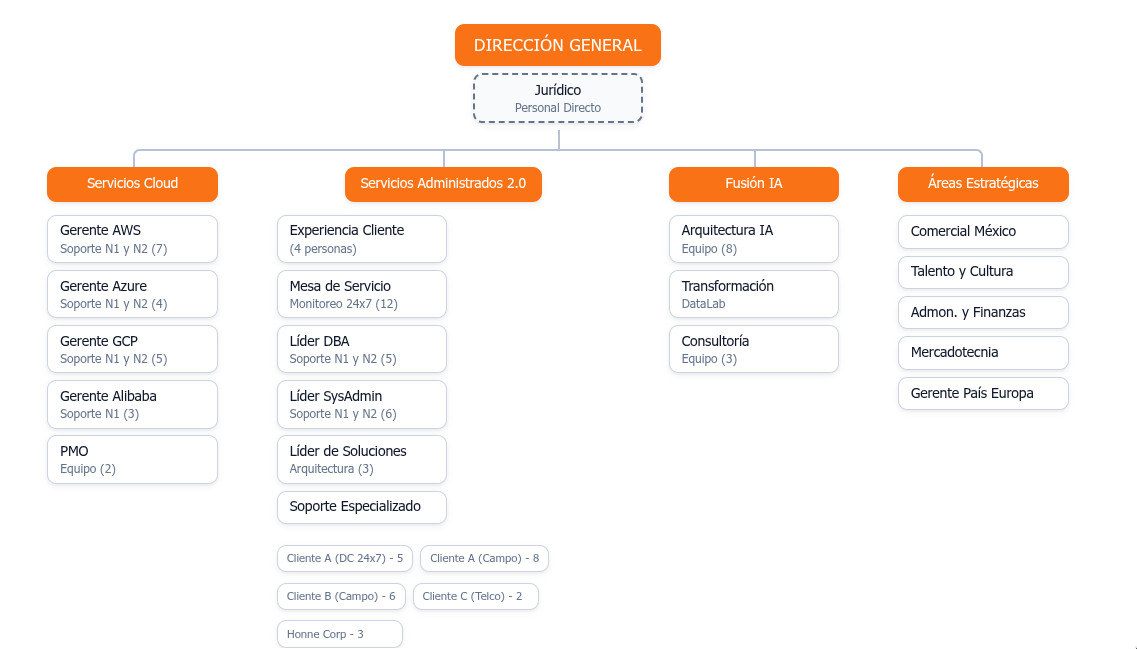
\includegraphics[width=0.8\textwidth]{img/figura_organigrama.png}
    \caption{Organigrama de Honne, con la Mesa de Servicio dentro de Servicios Administrados 2.0.}
    \label{fig:organigrama}
\end{figure}


\subsection{Descripción del área de trabajo y sus funciones}
\label{sec:area_trabajo}

El área en la que se realizó la Estadía es la Mesa de Servicio del CCoE. Su función principal es atender las solicitudes de los clientes relacionadas con sus instancias en la nube (AWS, Google Cloud Platform y Microsoft Azure), bases de datos y demás recursos de infraestructura, así como identificar errores o fallas en esas instancias y reportarlos a los usuarios para que soliciten su corrección.

La operación del área combina distintos canales y herramientas de trabajo. El correo electrónico de soporte técnico para el cliente es el canal principal para recibir alertas de errores e incidencias generadas por los distintos proveedores de cómputo en la nube. Además, para clientes específicos se emplean plataformas de monitoreo dedicadas como ServiceNow y TIBCO Scribe, mientras que Zendesk se utiliza principalmente para la gestión y asignación de tickets a las áreas responsables de la corrección de errores, como SysAdmin.

Los tickets atendidos abarcan una variedad de solicitudes de infraestructura y soporte, tales como la activación de autenticación multifactor (MFA), el restablecimiento de contraseñas, el ajuste de husos horarios, la validación de respaldos, la baja de usuarios, la asistencia en sesiones de trabajo y la elaboración de reportes periódicos de facturación, entre otros.

Como apoyo adicional, el área utiliza bots que automatizan parte del monitoreo, enviando notificaciones a través de Telegram sobre el estado de los servidores y la llegada de nuevos tickets en Zendesk.
